\phantomsection
\chapter{Valutazione Sperimentale}
\markboth{Valutazione Sperimentale}{}
\label{cap5:valutazione_sperimentale}
% [titolo ridotto se non ci dovesse stare]
\section{Valutazione della metafora}
La metafora di visualizzazione descritta precedentemente \`{e} stata valutata \cite{mdvisualization} in uno studio qualitativo sottoposto ad utenti esperti, ovvero studenti del dottorato di ricerca ed amministratori di database, poich\'{e} l'obiettivo era valutare i task di analisi esplorativa, per i quali gli studi qualitativi si sono dimostrati pi\`{u} adatti delle misure quantitative \cite{informationvisualization,strategies4evaluatinginfo}. In particolare, lo studio \`{e} stato svolto con sei utenti in una sessione di due ore, nella quale gli utenti hanno utilizzato la metafora proposta con tre dataset pubblici tratti dalla repository della UCI Machine Learning \cite{ucirepository}: Breast-cancer, Bridges e Echocardiogram. Le statistiche delle caratteristiche dei dataset considerati ed il numero di \acrshort{rfds} trovate sono riportate nella Tabella \ref{table:1},
% -- Tabella dei risultati
\begin{table}[h!]
\centering
%\refstepcounter{table}
\begin{tabular}{|l|rrrr|r|} 
\hline
\multicolumn{1}{|c|}{\multirow{2}{*}{\textbf{Dataset}}} & \multicolumn{4}{c|}{\textbf{Statistiche}}                                                                                              & \multicolumn{1}{c|}{\multirow{2}{*}{\textbf{\#RFD Totali}}}  \\
\multicolumn{1}{|c|}{}                         & \multicolumn{1}{l}{\textbf{\#Colonne}} & \multicolumn{1}{l}{\textbf{\#Righe}} & \multicolumn{1}{l}{\textbf{\#FD}} & \multicolumn{1}{l|}{\textbf{Dimensione (KB)}} & \multicolumn{1}{c|}{}                                \\ 
\hline
Breast-cancer                                  & 11                            & 699                         & 46                       & 20                                   & 814                                                  \\
Bridges                                        & 13                            & 107                         & 142                      & 6                                    & 6960                                                 \\
Echocardiogram                                 & 13                            & 132                         & 538                      & 6                                    & 2396                                                 \\
\hline
\end{tabular}
\caption{Statistiche e risultati delle RFD scoperte sui dataset considerati.}
\label{table:1}
\end{table}
% -- Fine Tabella
mentre la metafora di visualizzazione applicata al dataset Echocardiogram \`{e} mostrata in Figura \ref{fig:colored_matrix_echo}.
% -- Metafora per le RFDs scovate in Echocardiogram
\begin{figure}[ht]
    \centering
    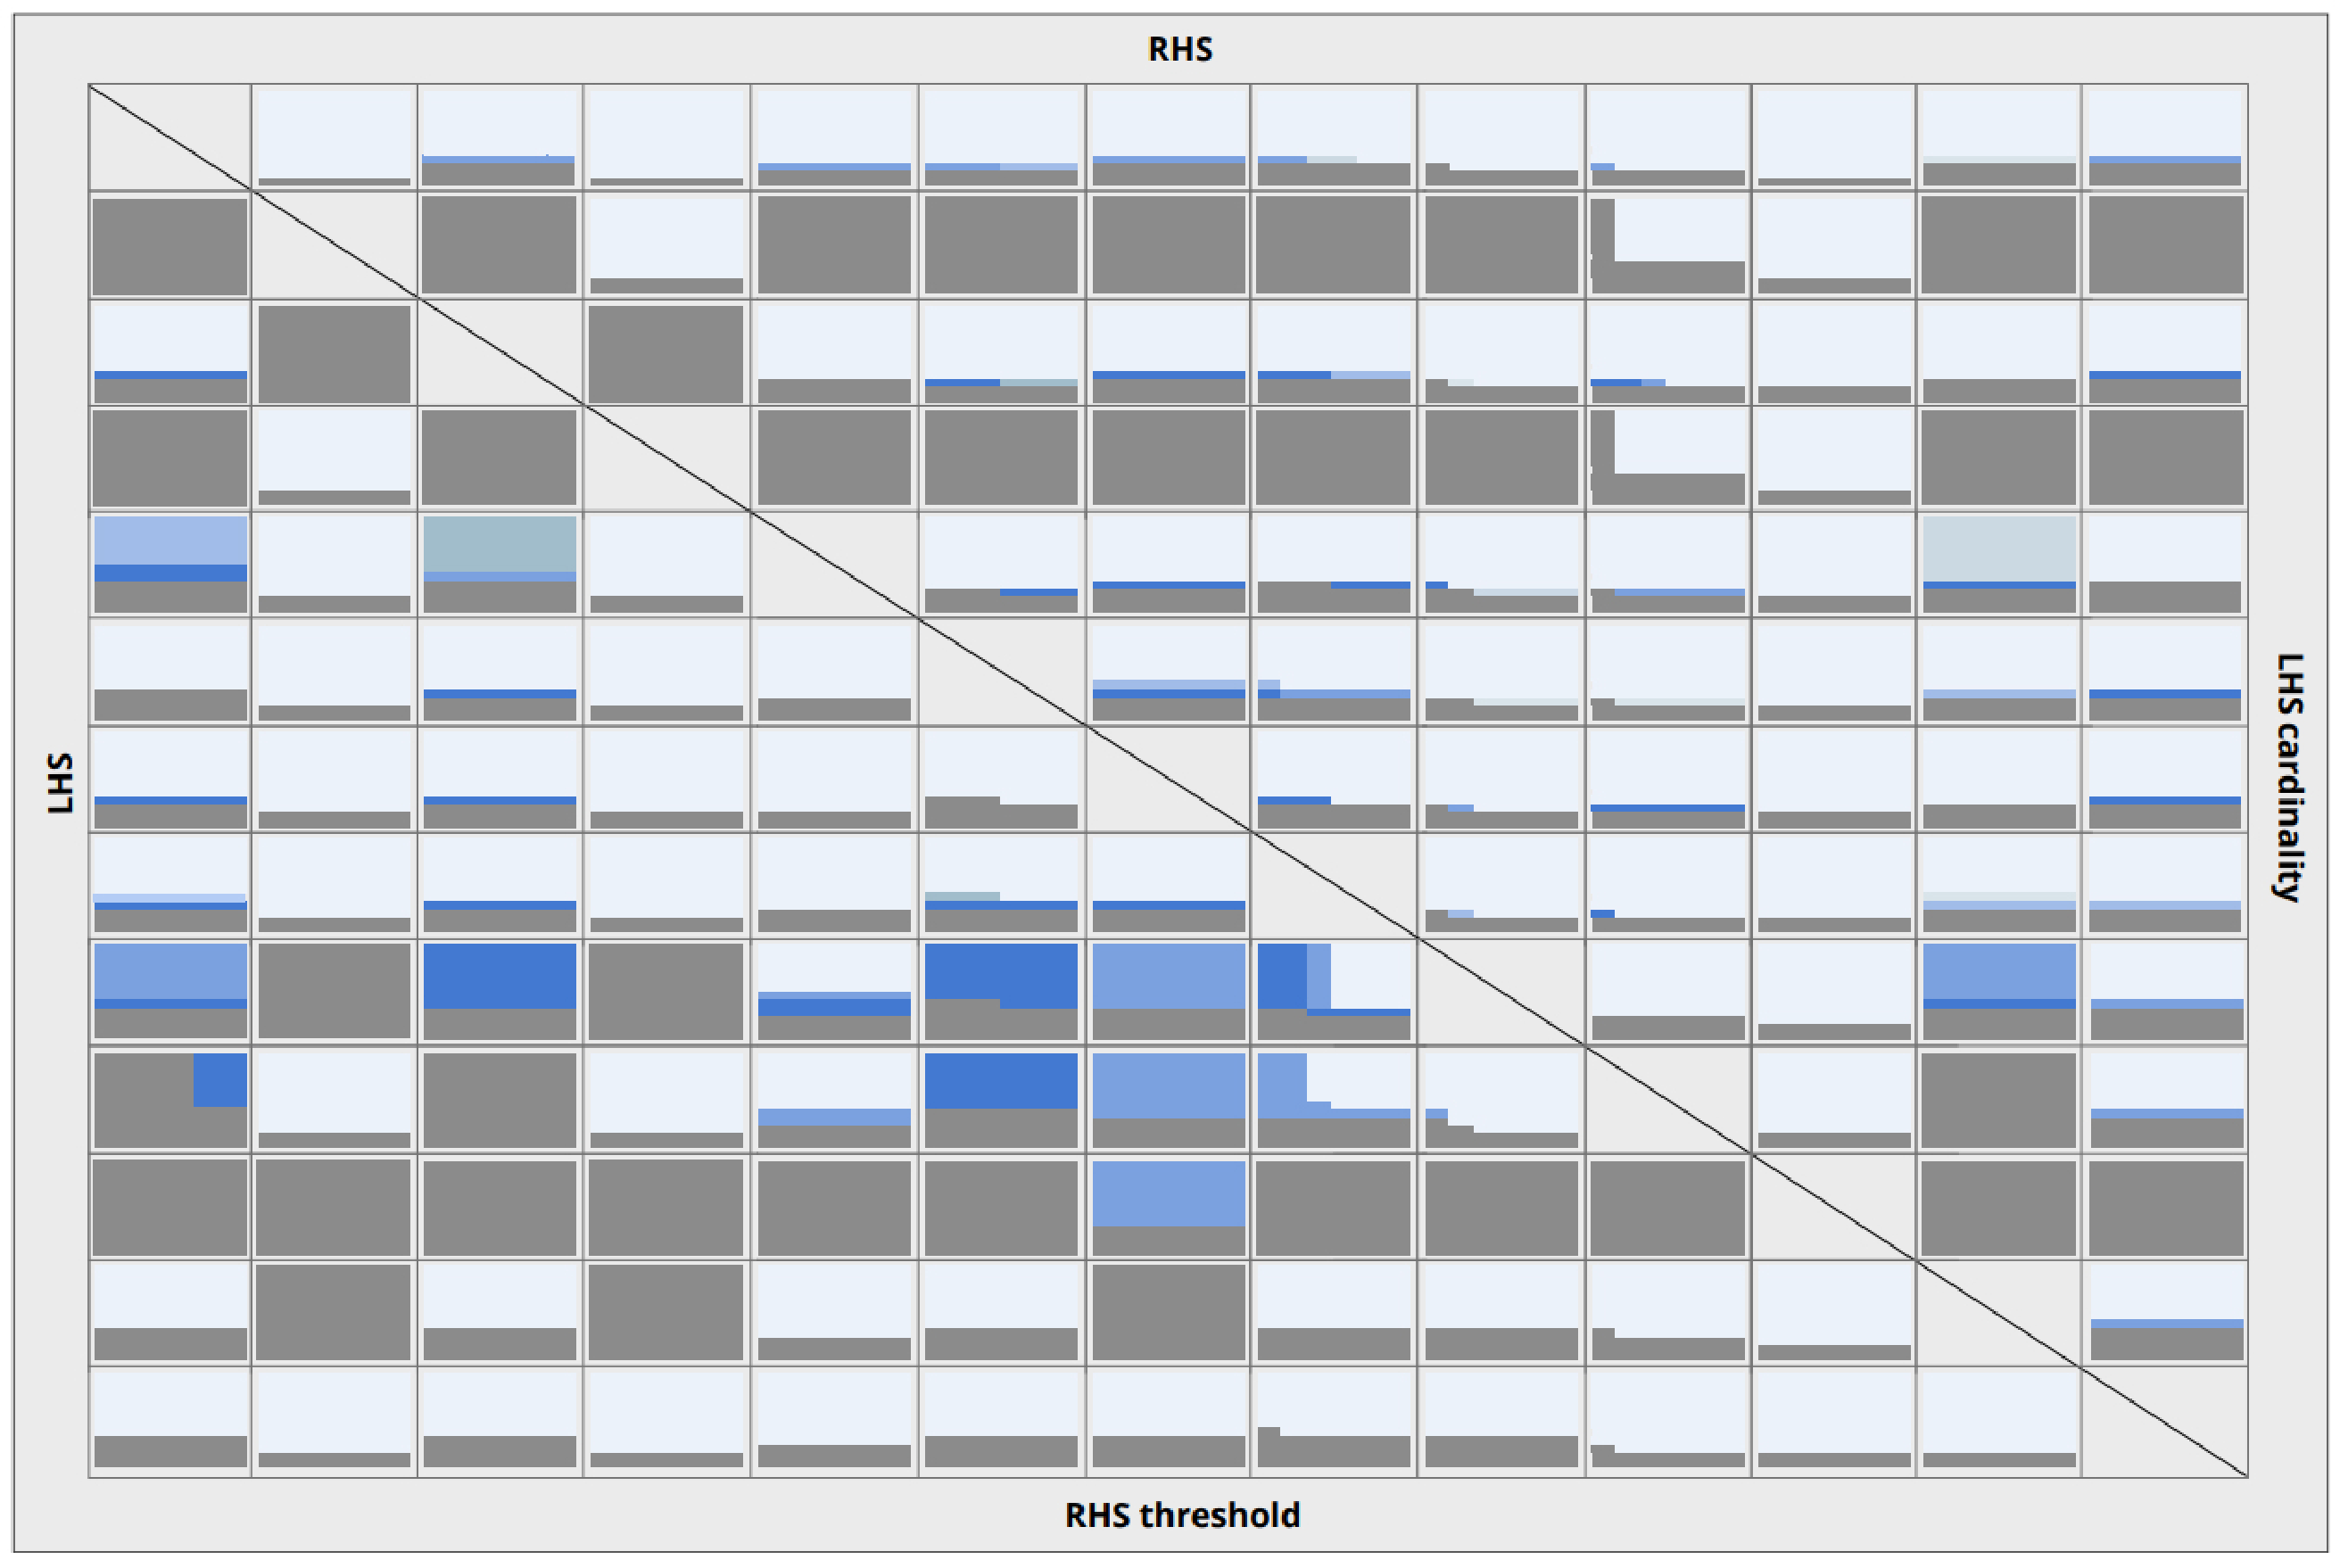
\includegraphics[width=\linewidth]{capitoli/figure/echo_metaphore}
    \caption{Matrice colorata per le \acrshort{rfds} estratte dal dataset Echocardiogram.}
    \label{fig:colored_matrix_echo}
\end{figure}
% -- Fine metafora
Al termine della sessione di valutazione, questi erano i feedback degli utenti in merito ai vantaggi delle metafore di visualizzazione proposte:
\begin{itemize}
    \item \textit{Coinvolgimento degli attributi nelle \acrshort{rfds}}: oltre alla frequenza con cui un attributo si presenta nelle \acrshort{rfds}, la matrice colorata ha fornito informazioni sulla loro frequenza di occorrenza sul lato sinistro o sul lato destro, affermando se un attributo \`{e} pi\`{u} implicato da un altro attributo oppure implica altri attributi;
    \item \textit{Cardinalit\`{a} del lato sinistro}: mentre la cardinalit\`{a} del lato destro delle \acrshort{rfds} trovate \`{e} sempre pari a $1$, quella del lato sinistro pu\`{o} variare tra $1$ ed il numero di attributi meno $1$. La matrice colorata fornisce un feedback immediato sulla cardinalit\`{a} del lato sinistro;
    \item \textit{Correlazione degli attributi}: per un dato attributo sul lato destro, tutti gli utenti hanno concordato sul fatto che la matrice colorata ha fornito un feedback immediato sulle correlazioni degli attributi, ovvero con quale frequenza due attributi si trovano su lati diversi della stessa \acrshort{rfd};
\end{itemize}
In sintesi, l'analisi della metafora proposta rivela che ha supportato con successo utenti esperti nell'analisi di enormi set di \acrshort{rfds} e le loro soglie associate. Soprattutto, ha fornito nuove panoramiche e astrazioni delle \acrshort{rfds} scoperte, riducendo considerevolmente lo sforzo necessario per analizzarle.

\section{Risultati}
Attraverso l'implementazione della metafora di visualizzazione esposta nel capitolo \ref{section:visual_rep_metaphore} all'interno di Dependensee, si \`{e} riusciti a rappresentare in modo immediato ed efficace un dataset di \acrlong{rfds} minimali. In questo modo \`{e} stato possibile effettuare un'analisi visiva quasi istantanea, grazie alle diverse caratteristiche messe in luce dalla rappresentazione grafica fornita dallo strumento. Infatti, questa rappresentazione raffigura le dipendenze minimali esistenti tra tutti gli attributi contenute nel dataset, mettendo in risalto la cardinalit\`{a} del lato sinistro e le soglie associate sia per il lato sinistro che per il lato destro.\par
% -- TAB DATASET --
\begin{table}[ht]
\centering
\begin{tabular}{|lrrr|} 
\hline
\multicolumn{4}{|c|}{\textbf{Statistiche}}                                                                                                \\
\textbf{Dataset} & \multicolumn{1}{c}{\textbf{\#Attributi}} & \multicolumn{1}{c}{\textbf{\#Tuple}} & \multicolumn{1}{l|}{\textbf{\#RFD}}  \\ 
\hline
Echocardiogram   & 13                                       & 132                                    & 2396                                 \\
Citiseer   & 7                                        & 2000                                    & 107                                  \\
Car\_data        & 7                                        & 1729                                    & 8                                    \\
Restaurant       & 6                                        & 864                                    & 1961                                 \\
Foodstamp        & 5                                        & 150                                    & 9                                    \\
expIDEAS         & 3                                        & 7                                    & 12                                   \\
\hline
\end{tabular}
\caption{Statistiche dei dataset analizzati con Dependensee.}
\label{table:datasets_analyzed_stats}
\end{table}
% -- END TAB DATASET --
La valutazione \`{e} avvenuta attraverso l'analisi dei dataset elencati nella Tabella \ref{table:datasets_analyzed_stats}, i quali presentano caratteristiche differenti, come il numero di attributi, il numero di tuple ed il numero di \acrshort{rfds} individuate.
\begin{figure}[ht]
    \centering
    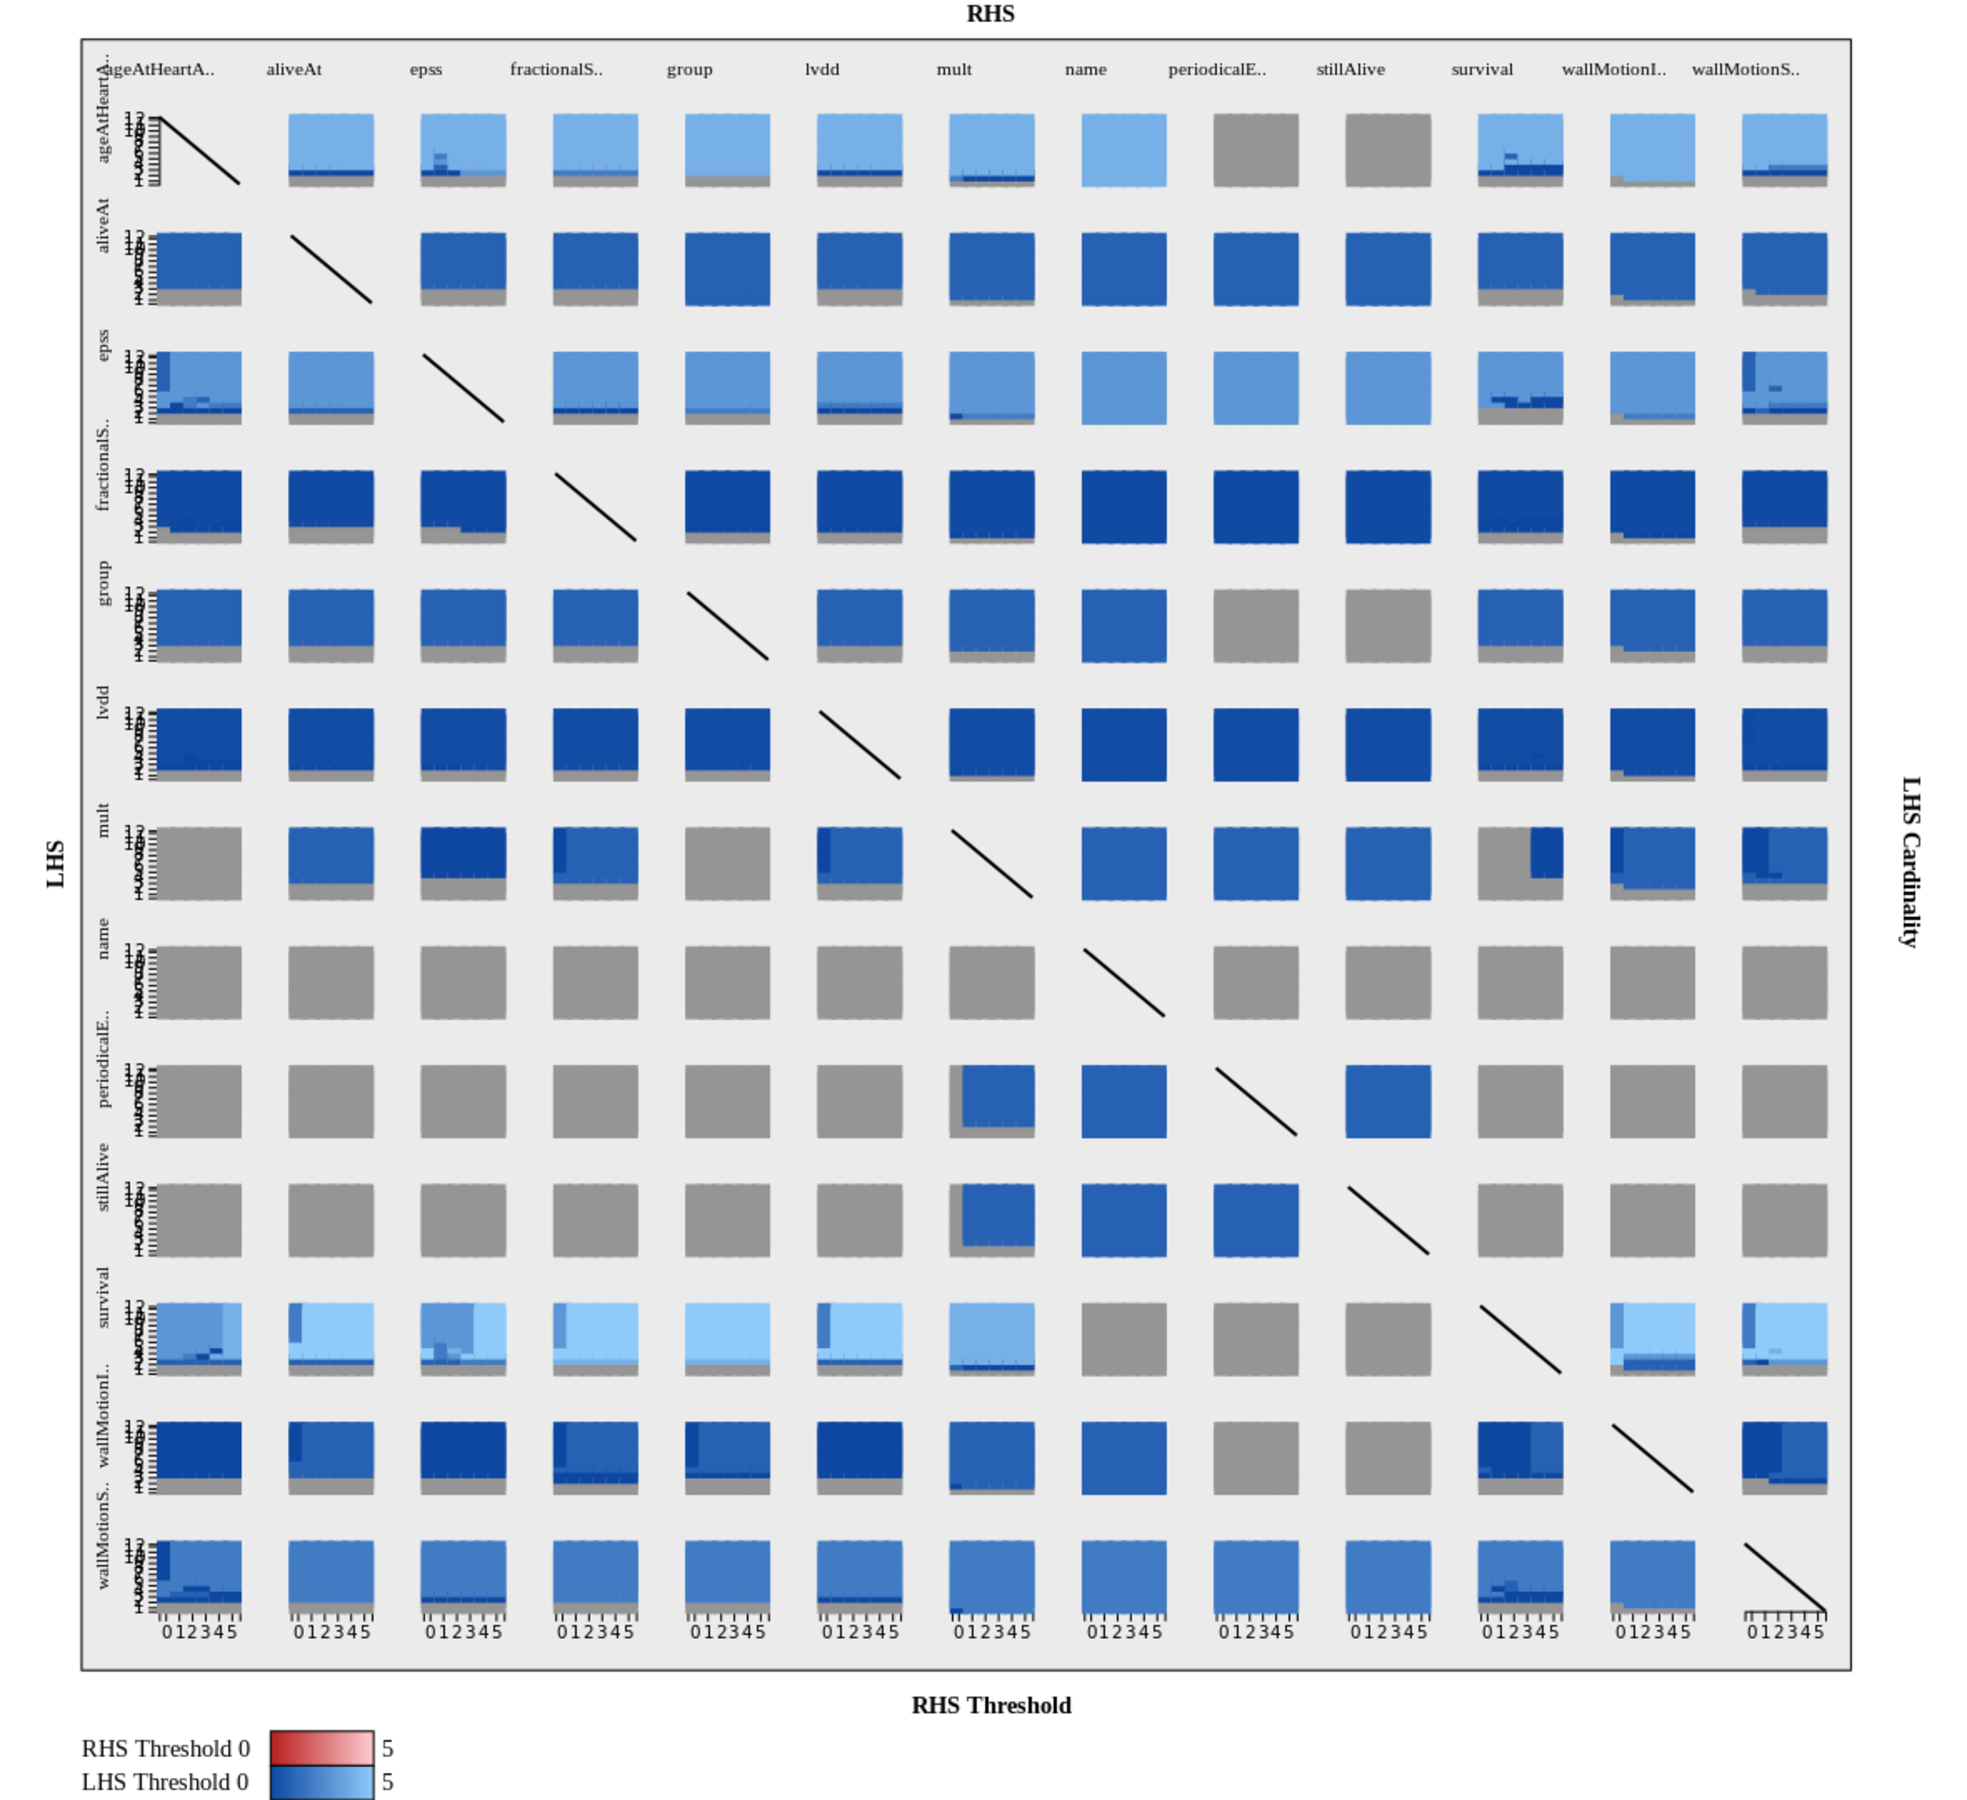
\includegraphics[width=\linewidth]{capitoli/figure/echocardiogram}
    \caption{Rappresentazione ottenuta in output da Dependensee del dataset Echocardiogram.}
    \label{fig:echocardiogram_result}
\end{figure}
La Figura \ref{fig:echocardiogram_result} mostra la grafica ottenuta analizzando il dataset \textit{Echocardiogram} con Dependensee. Da un primo sguardo si pu\`{o} notare come questa faciliti effettivamente l'analisi visuale per l'utente. Analizzando il dataset attraverso tale rappresentazione possiamo notare, mediante la diagonale nulla, come le \acrlong{rfds} banali non vengano rappresentate. In questo caso, data la grande mole di attributi, il grafico risultante enfatizza la soglia del lato sinistro piuttosto che quella del lato destro, essendo quest'ultima fissata. Inoltre, le label di alcuni attributi vengono troncate in quanto troppo lunghe, per evitare che queste si sovrappongano alle altre label. Il dataset \`{e} stato analizzato con una soglia massima data in input pari a $5$ e la gran parte delle \acrlong{rfds} minimali hanno la soglia minima o un valore vicino al minimo sul lato sinistro, poche con una soglia di valore massimo. Dalla Figura \ref{fig:echocardiogram_result} possiamo notare che non esistono \acrlong{rfds} minimali con l'attributo \texttt{name} sul lato sinistro con soglia tra $0$ e $5$, in quanto tutta la riga \`{e} di color grigio. Se osserviamo, invece, la prima riga e la seconda colonna, possiamo notare l'esistenza di \acrlong{rfds} minimali di cardinalit\`{a} $3$ con soglia minima e le \acrlong{rfds} minimali con cardinalit\`{a} maggiore sono tutte con soglia massima. Se consideriamo la riga con l'attributo \texttt{ageAtHearthAttack} sul lato sinistro e la colonna con l'attributo \texttt{name} sul lato destro, ovvero prima riga ed ottava colonna, possiamo notare che tutte le \acrlong{rfds} minimali sono con soglia massima pari a $5$, difatti tutta la sotto-matrice presenta il colore pi\`{u} chiaro. Da un'analisi generale, invece, si pu\`{o} notare che la gran parte delle \acrlong{rfds} minimali sono con soglia minima pari a $0$, molte con soglia di valore medio tra $1$ e $4$, poche con soglia pari al valore massimo $5$.\par
\begin{figure}[ht]
    \centering
    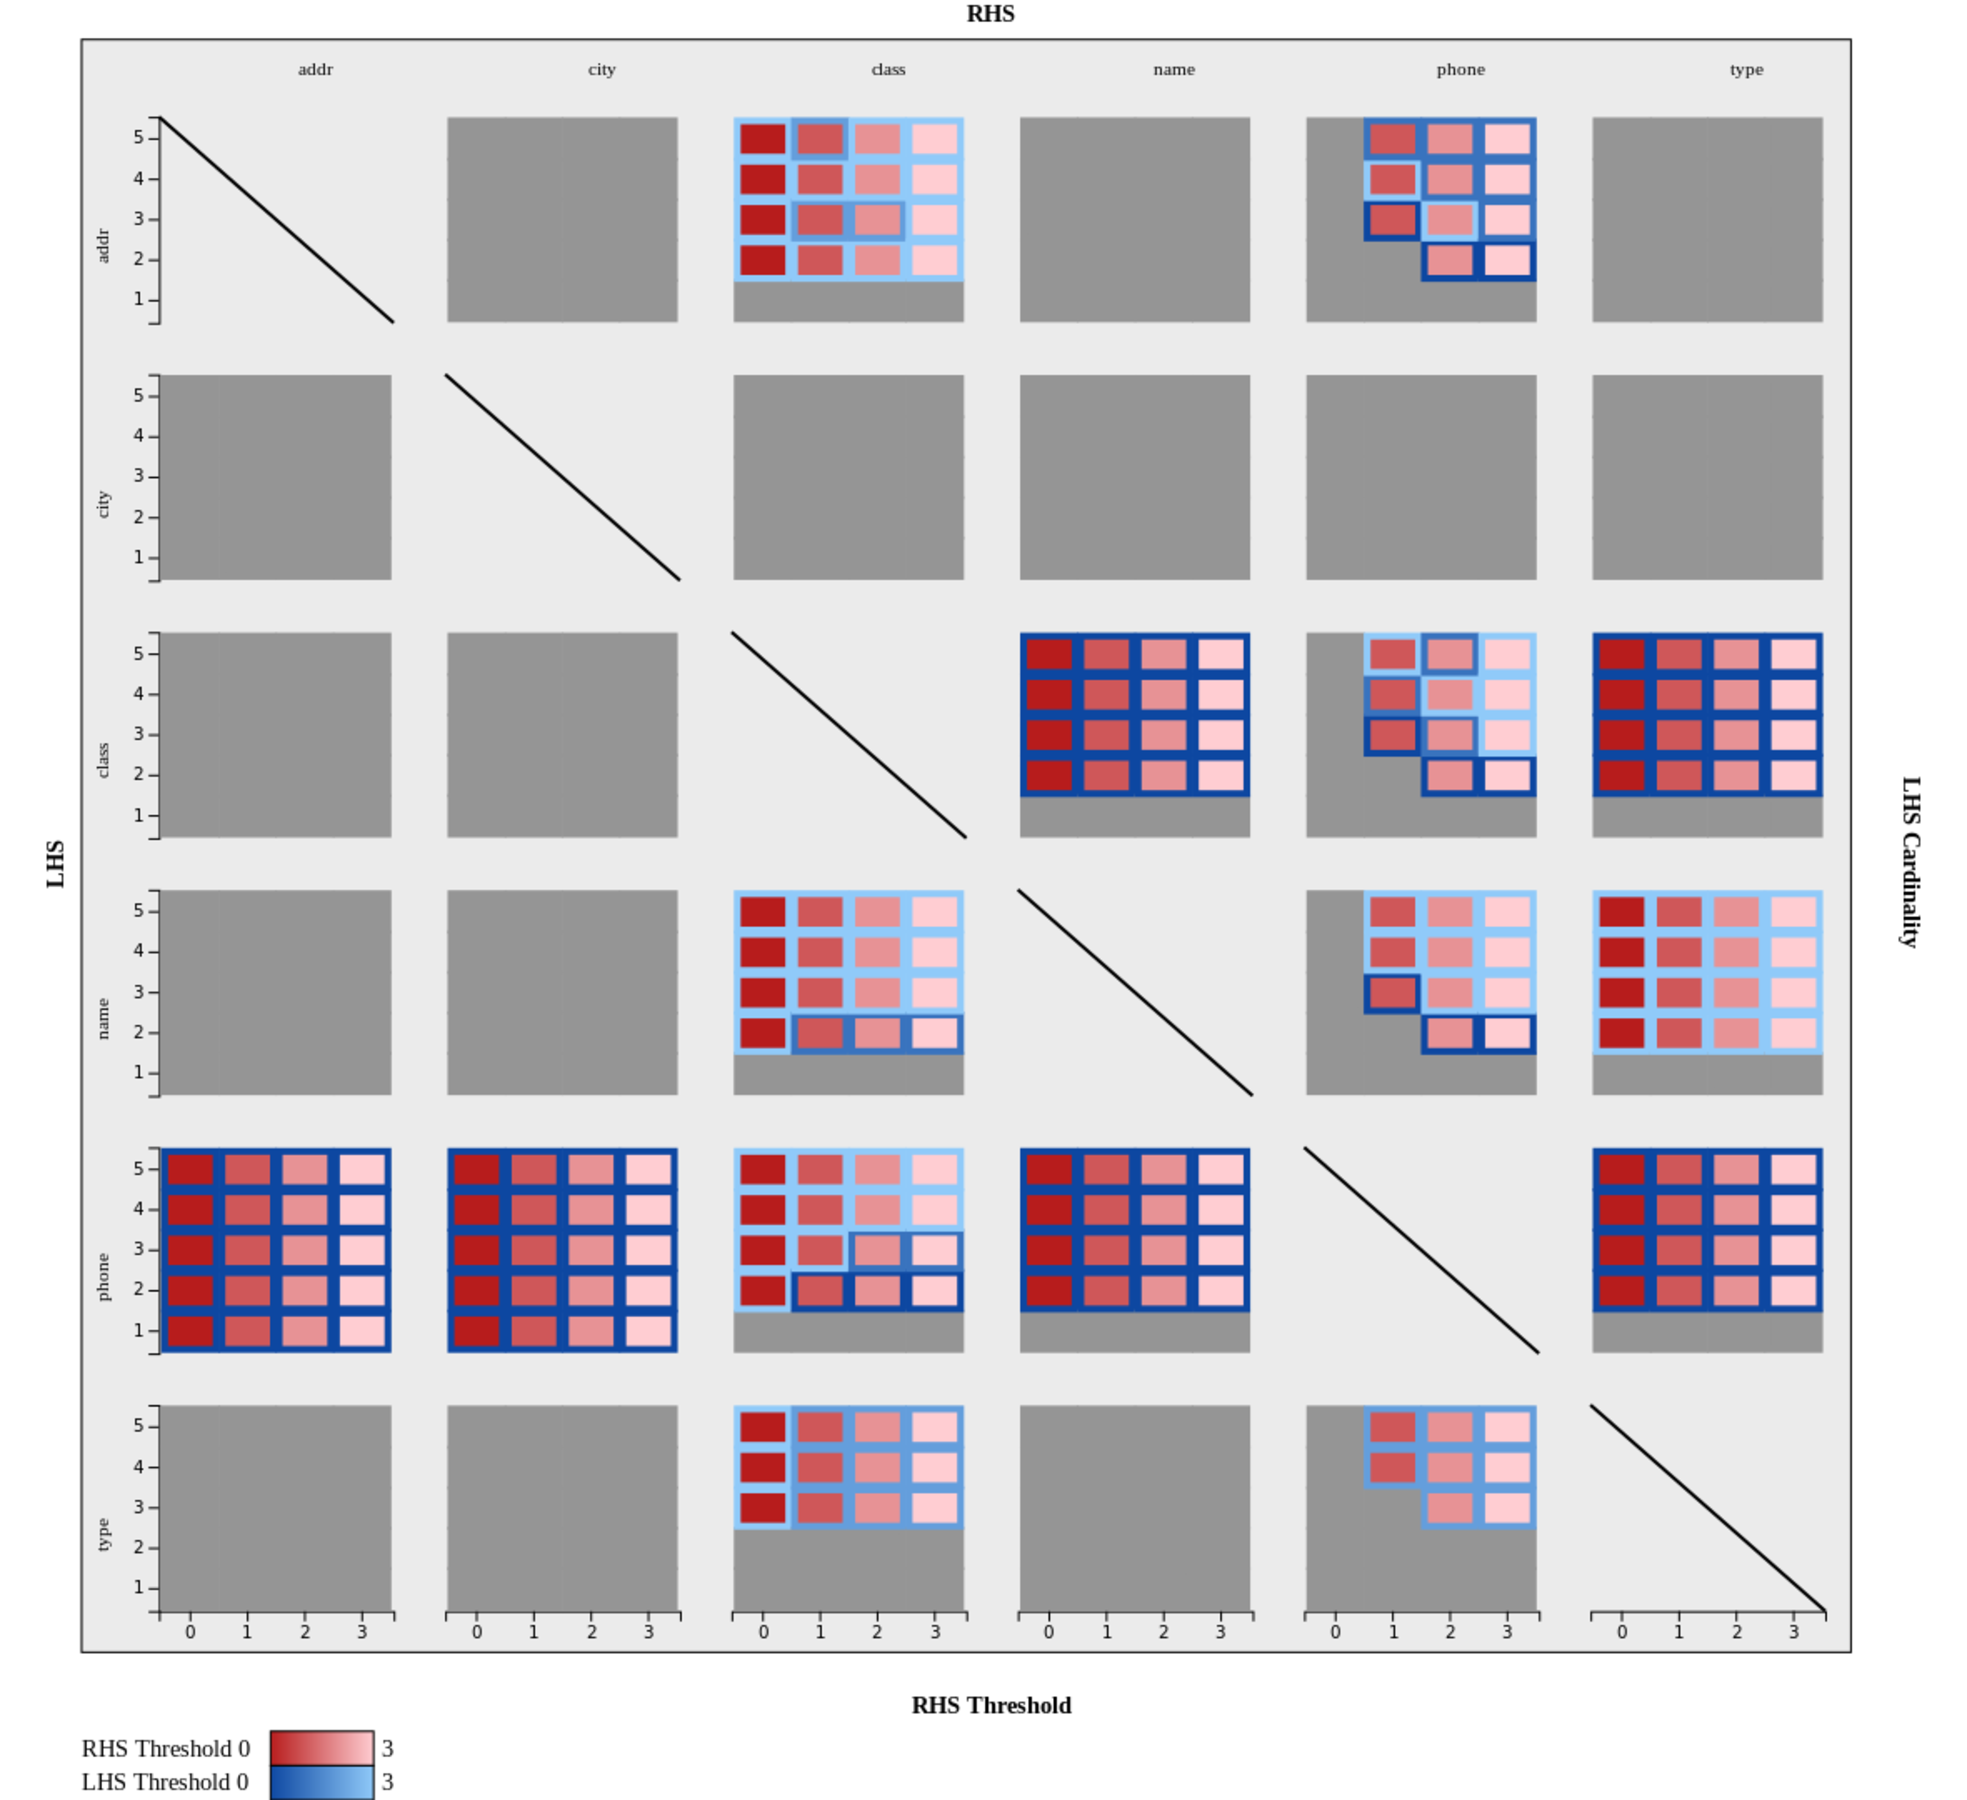
\includegraphics[width=\linewidth]{capitoli/figure/restaurant}
    \caption{Rappresentazione ottenuta in output da Dependensee del dataset Restaurant.}
    \label{fig:restaurant_result}
\end{figure}
Per quanto concerne l'analisi del dataset \textit{Restaurant}, la Figura \ref{fig:restaurant_result} mostra la rappresentazione grafica ottenuta mediante l'utilizzo di Dependensee. Da un'analisi generale si pu\`{o} affermare che le \acrlong{rfds} minimimali esistenti sono distribuite e non coprono tutti gli attributi del dataset. Infatti, la seconda riga \`{e} totalmente grigia, segno che non esiste alcuna \acrlong{rfds} minimale con l'attributo \texttt{city} sul lato sinistro. Continuando, vi sono molte altre sotto-matrici grigie che indicano l'assenza di \acrlong{rfds} minimali. Ci\`{o} non \`{e} uguale per tutte le sotto-matrici del grafico. Se consideriamo la riga relativa all'attributo \texttt{phone}, questa presenta \acrlong{rfds} minimali per tutti gli attributi. Le \acrlong{rfds} minimali con l'attributo \texttt{phone} sul lato sinistro, in relazione con gli attributi \texttt{addr}, \texttt{city}, \texttt{name} e \texttt{type} sul lato destro, sono tutte soglia minima sul lato sinistro. Mentre, la maggior parte di quelle in relazione con l'attributo \texttt{class} sul lato destro hanno soglia massima, alcune hanno soglia minima o quasi. Se, invece, consideriamo la terza colonna relativa all'attributo \texttt{class} sul lato destro, possiamo notare che quasi tutte le \acrlong{rfds} minimali hanno soglia massima o molto vicina a questa sul lato sinistro. Invece, la colonna relativa all'attributo \texttt{addr} sul lato destro, presenta solo \acrlong{rfds} minimali con soglia minima sul lato sinistro in relazione con l'attributo \texttt{phone}. Considerando, invece, la colonna relativa all'attributo \texttt{name} sul lato destro, presenta solo \acrlong{rfds} minimali con soglia minima sul lato sinistro relative agli attributi \texttt{class} e \texttt{phone}. Invece, l'ultima colonna relativa all'attributo \texttt{type} presenta \acrlong{rfds} minimali solo con gli attributi \texttt{class}, \texttt{name} e \texttt{phone}. Quelle relative agli attributi \texttt{class} e \texttt{phone} sul lato destro sono tutte con soglia minima, mentre quelle relative all'attributo \texttt{name} sono tutte con soglia massima.\par
\begin{figure}[ht]
    \centering
    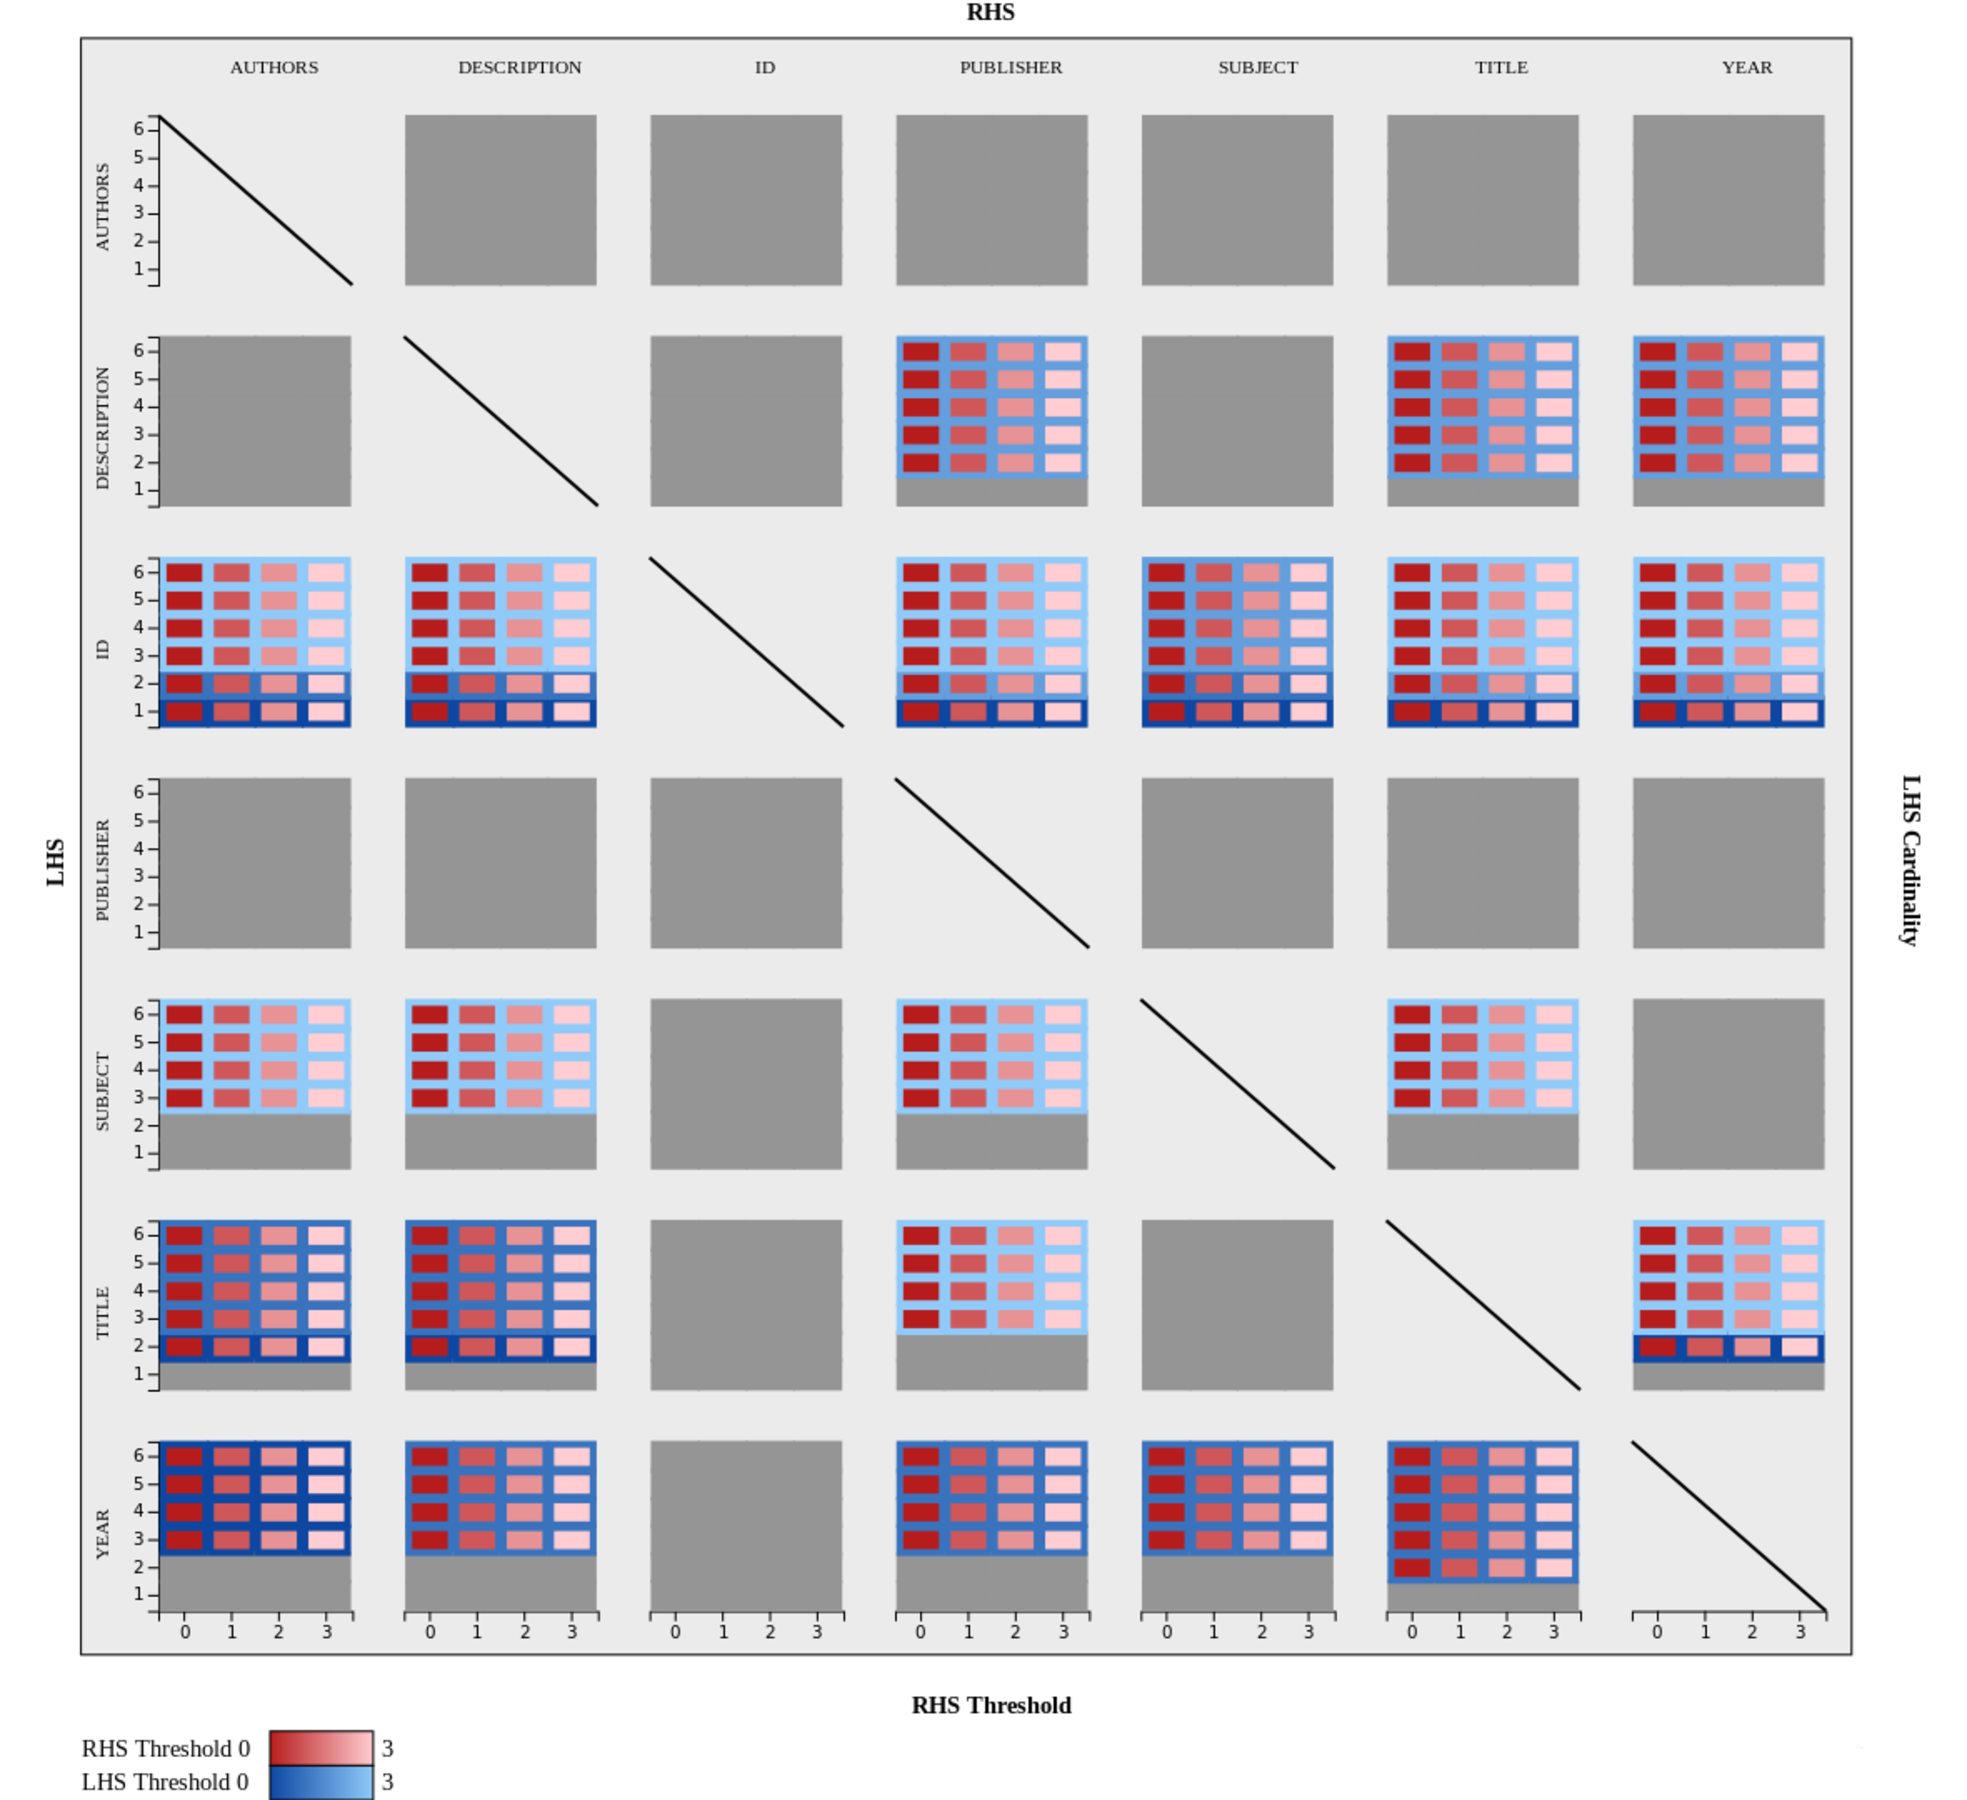
\includegraphics[width=\linewidth]{capitoli/figure/citiseer_2000_result}
    \caption{Rappresentazione ottenuta in output da Dependensee del dataset Citiseer.}
    \label{fig:citiseer_2000_result}
\end{figure}
La Figura \ref{fig:citiseer_2000_result} mostra la rappresentazione grafica ottenuta analizzando il dataset \textit{Citiseer} con Dependensee. Visto il basso numero di attributi, il grafico mostrer\`{a} anche il colore di riempimento relativo alla soglia del lato destro. Se prendiamo in considerazione la prima riga, possiamo notare come non esistano \acrlong{rfds} minimali con l'attributo \texttt{AUTHORS} sul lato sinistro e con almeno un attributo diverso sul lato destro, infatti tutta la riga \`{e} grigia. Analogamente con la terza riga, relativa all'attributo \texttt{PUBLISHER}. Mentre, con la colonna relativa all'attributo \texttt{ID}, possiamo notare l'assenza di \acrlong{rfds} minimali con l'attributo relativo sul lato destro. Se analizziamo la sotto-matrice relativa all'attributo riga \texttt{TITLE} ed all'attributo colonna \texttt{AUTHORS}, possiamo notare l'assenza di \acrlong{rfds} con cardinalit\`{a} pari a $1$ e l'esistenza di \acrlong{rfds} minimali con soglia pari a $0$ sul lato sinistro e cardinalit\`{a} pari a $2$, mentre per cardinalit\`{a} maggiori vi sono \acrlong{rfds} con soglia diverse da $0$ ma con valori vicini a questo.
Pi\`{u} in generale, la prima riga mostra l'esistenza di \acrlong{rfds} minimali con valore di soglia vicino al massimo inserito per l'analisi, ovvero $3$. La terza riga, invece, mostra la vasta presenza di \acrlong{rfds} minimali, molte con soglia pari al minimo o vicino a questo. La quinta riga, invece, mostra l'esistenza di \acrlong{rfds} minimali, tutte con valore di soglia minimo. L'ultima riga, invece, rappresenta le \acrshort{rfds} minimali, tutte con valore della soglia uguale al minino o vicino a questo.\par
\begin{figure}[H]
    \centering
    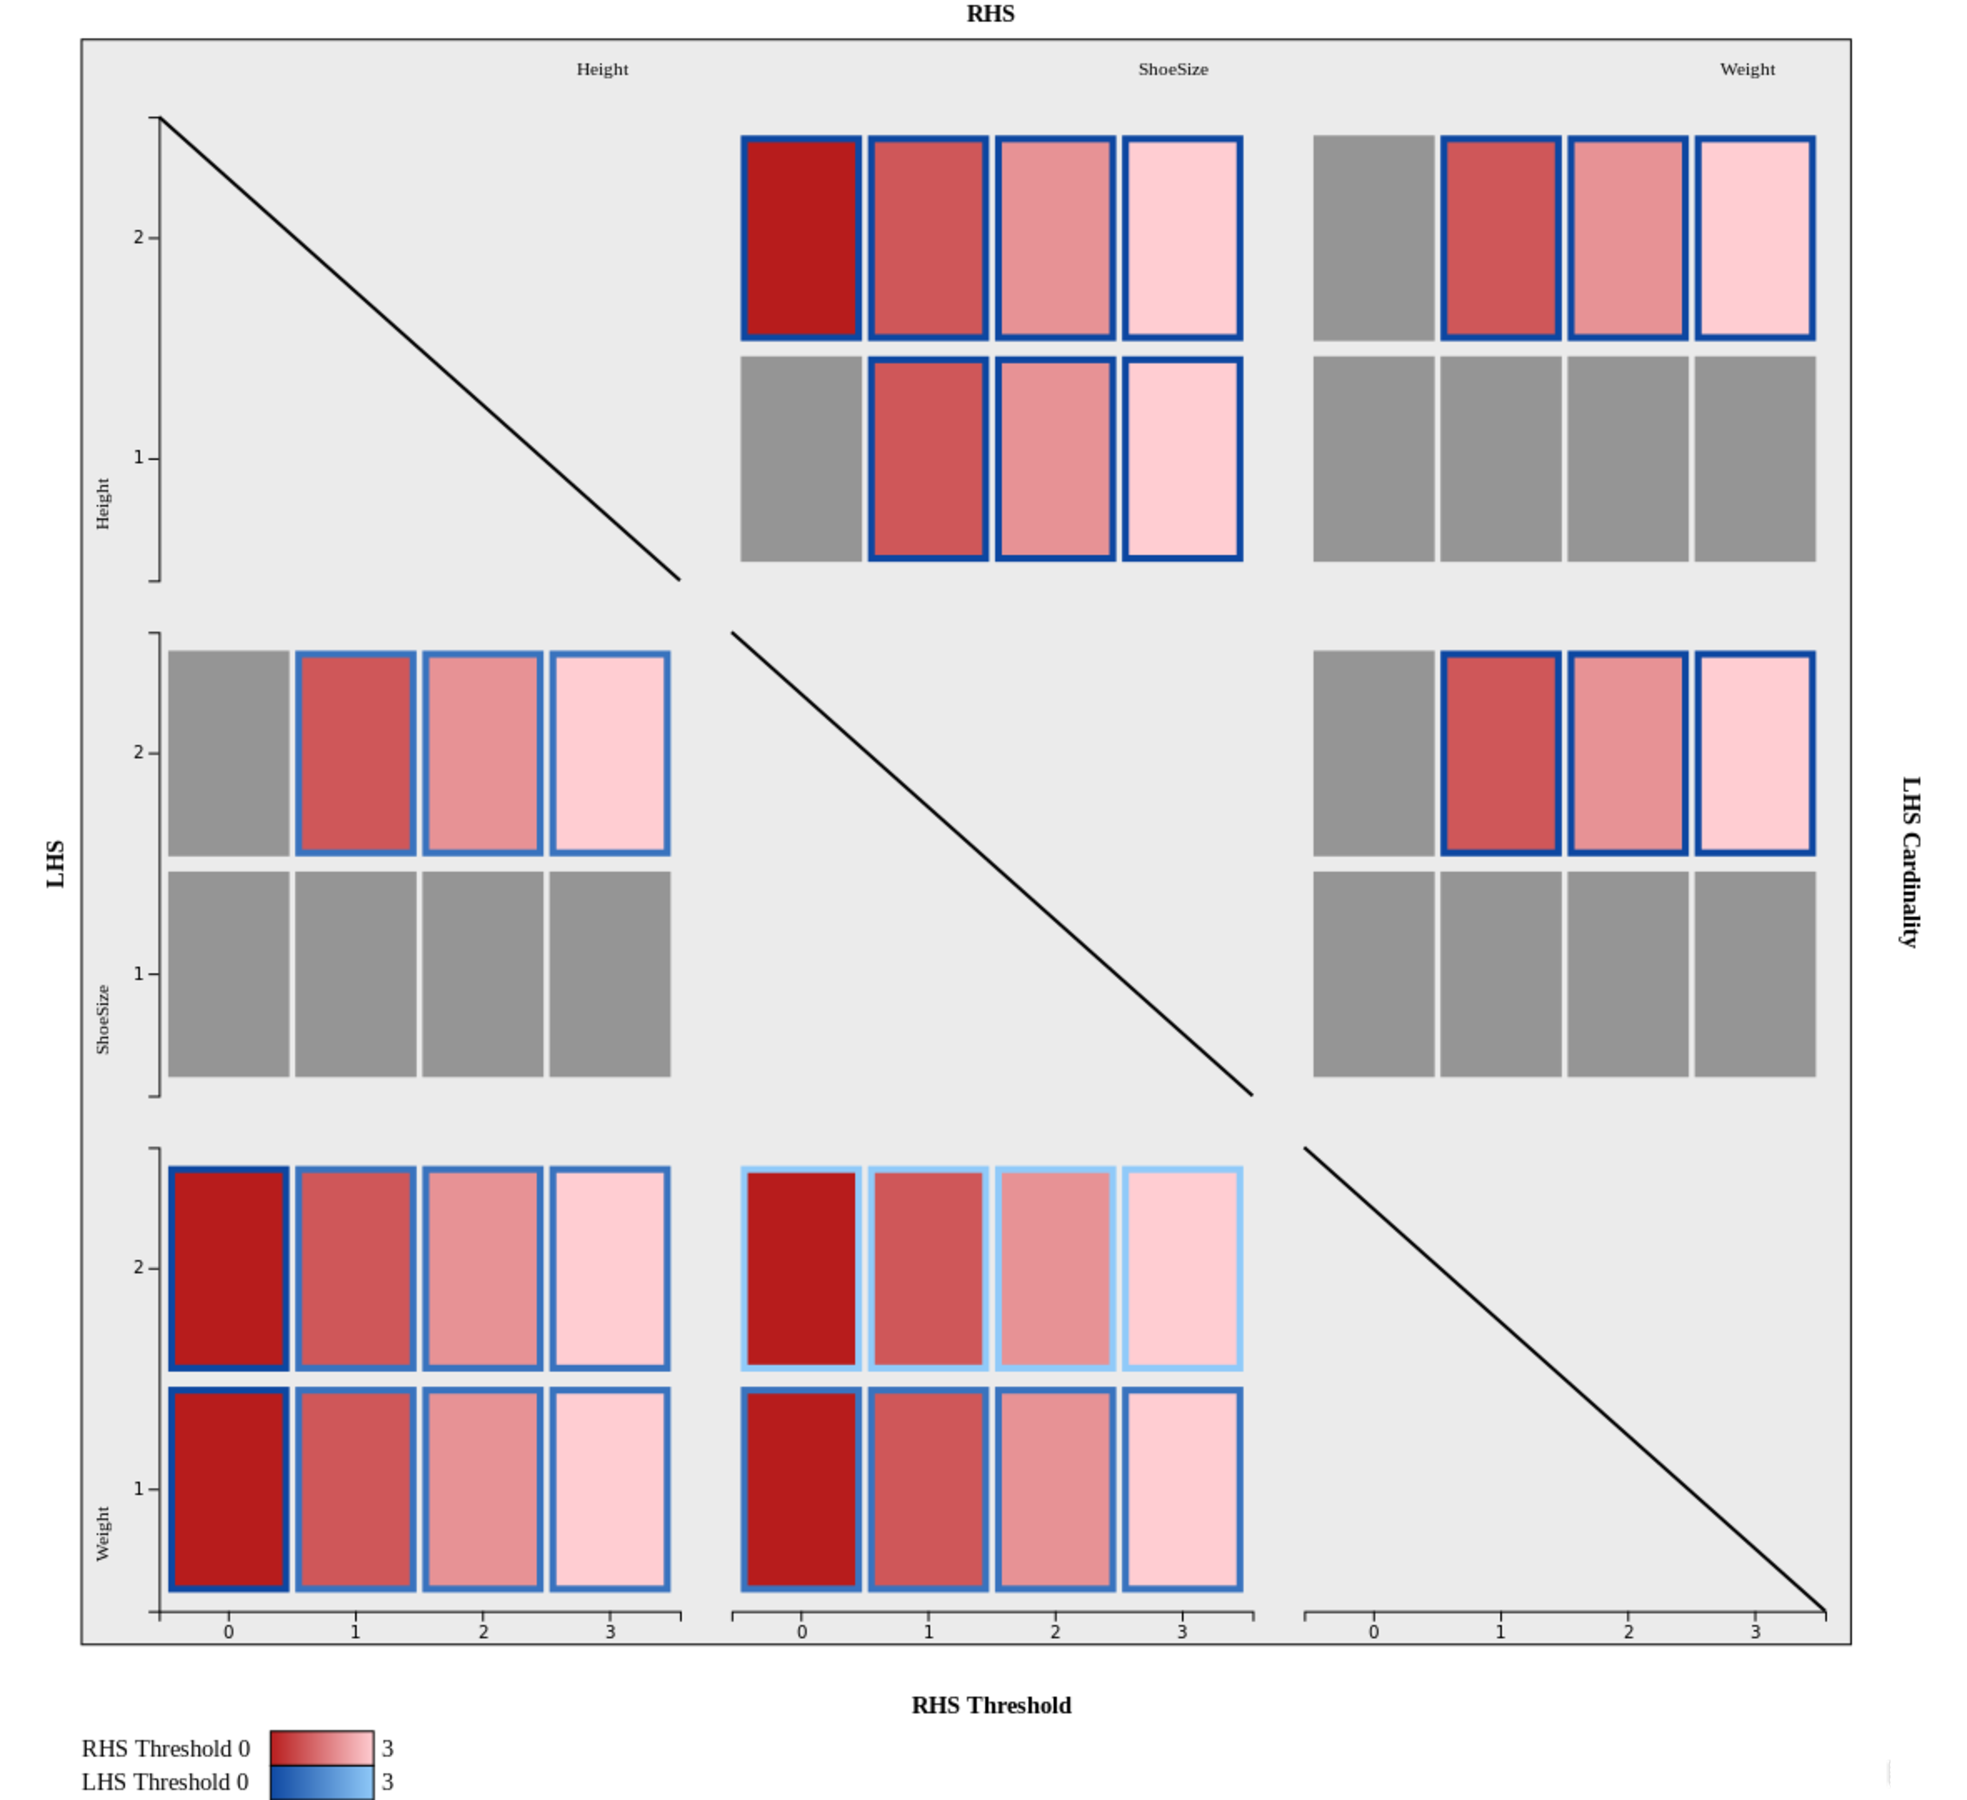
\includegraphics[width=\linewidth]{capitoli/figure/expIDEAS}
    \caption{Rappresentazione ottenuta in output da Dependensee del dataset expIDEAS.}
    \label{fig:expidea_result}
\end{figure}
La Figura \ref{fig:expidea_result} rappresenta il grafico ottenuto analizzando il dataset \textit{expIDEAS} mediante Dependensee. Il dataset contiene soltanto $3$ attributi e $12$ \acrlong{rfds} minimali. Dalla rappresentazione si pu\`{o} notare che le \acrlong{rfds} minimali sono ben distribuite. Con la prima riga possiamo notare che l'attributo \texttt{Height} sul lato sinistro figura in \acrlong{rfds} minimali con soglia minima. Anche con l'ultima colonna possiamo notare che l'attributo \texttt{Weight} sul lato destro figura in \acrlong{rfds} minimali con soglia minima. Invece, con l'ultima riga si pu\`{o} notare che l'attributo \texttt{Weight} sul lato sinistro figura in \acrlong{rfds} minimali, molte delle quali con soglia vicino o pari al massimo e poche con soglia pari al minimo.\par
\begin{figure}[ht]
    \centering
    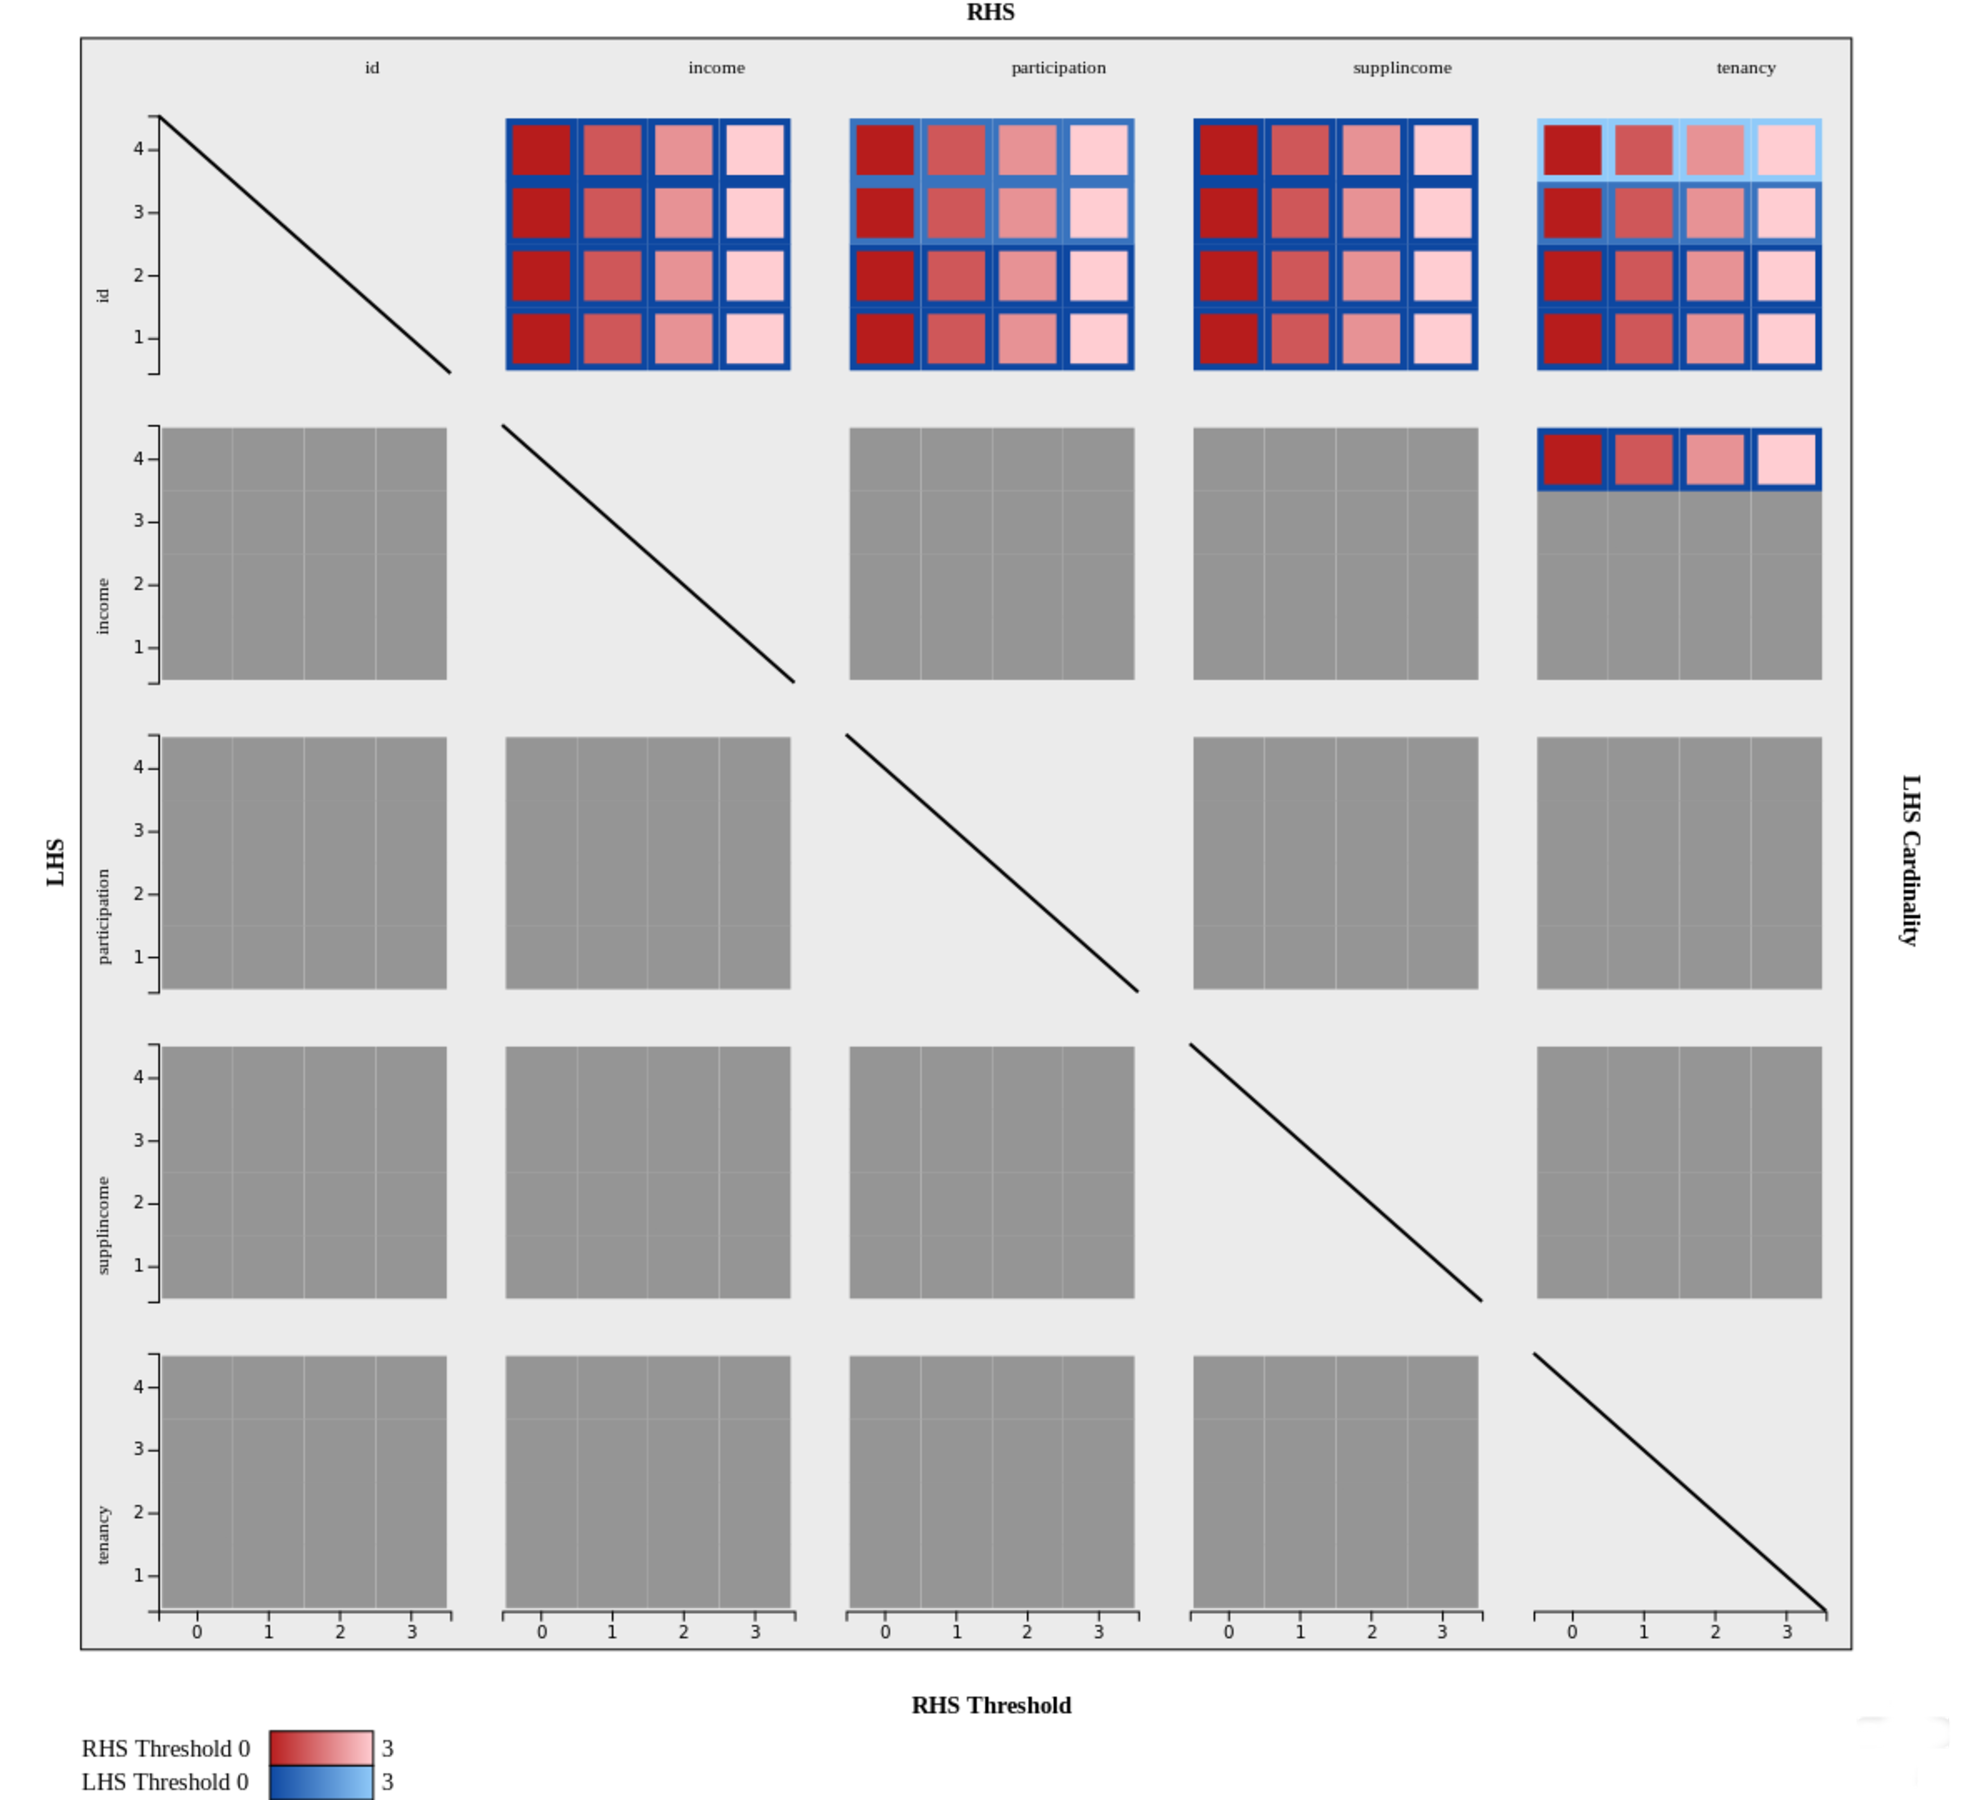
\includegraphics[width=\linewidth]{capitoli/figure/foodstamp_result}
    \caption{Rappresentazione ottenuta in output da Dependensee del dataset Foodstamp.}
    \label{fig:foodstamp_result}
\end{figure}
Consideriamo adesso il dataset \textit{Foodstamp}. La Figura \ref{fig:foodstamp_result} mostra la rappresentazione grafica ottenuta dando in input il dataset a Dependensee. Dal grafico ottenuto possiamo notare, attraverso la prima riga, come le uniche dipendenze esistenti siano con l'attributo \texttt{id} sul lato sinistro e, attraverso la seconda riga, con l'attributo \texttt{income} sul lato sinistro. Le prime sono in relazione con tutti gli altri attributi del dataset, infatti le colonne relative alla prima riga sono tutte colorate. Mentre, per l'attributo \texttt{income}, possiamo notare l'esistenza di \acrlong{rfds} solo con l'attributo \texttt{tenancy} sul lato destro. Le \acrlong{rfds} minimali presenti hanno quasi tutte una soglia minima o quasi, tranne quelle relative all'attributo \texttt{id} sul lato sinistro e l'attributo \texttt{tenancy} sul lato destro, le quali hanno soglia e cardinalit\`{a} massima. Con le righe e le colonne restanti possiamo notare che non vi sono \acrlong{rfds}, difatti sono colorate in grigio.\par
\begin{figure}[ht]
    \centering
    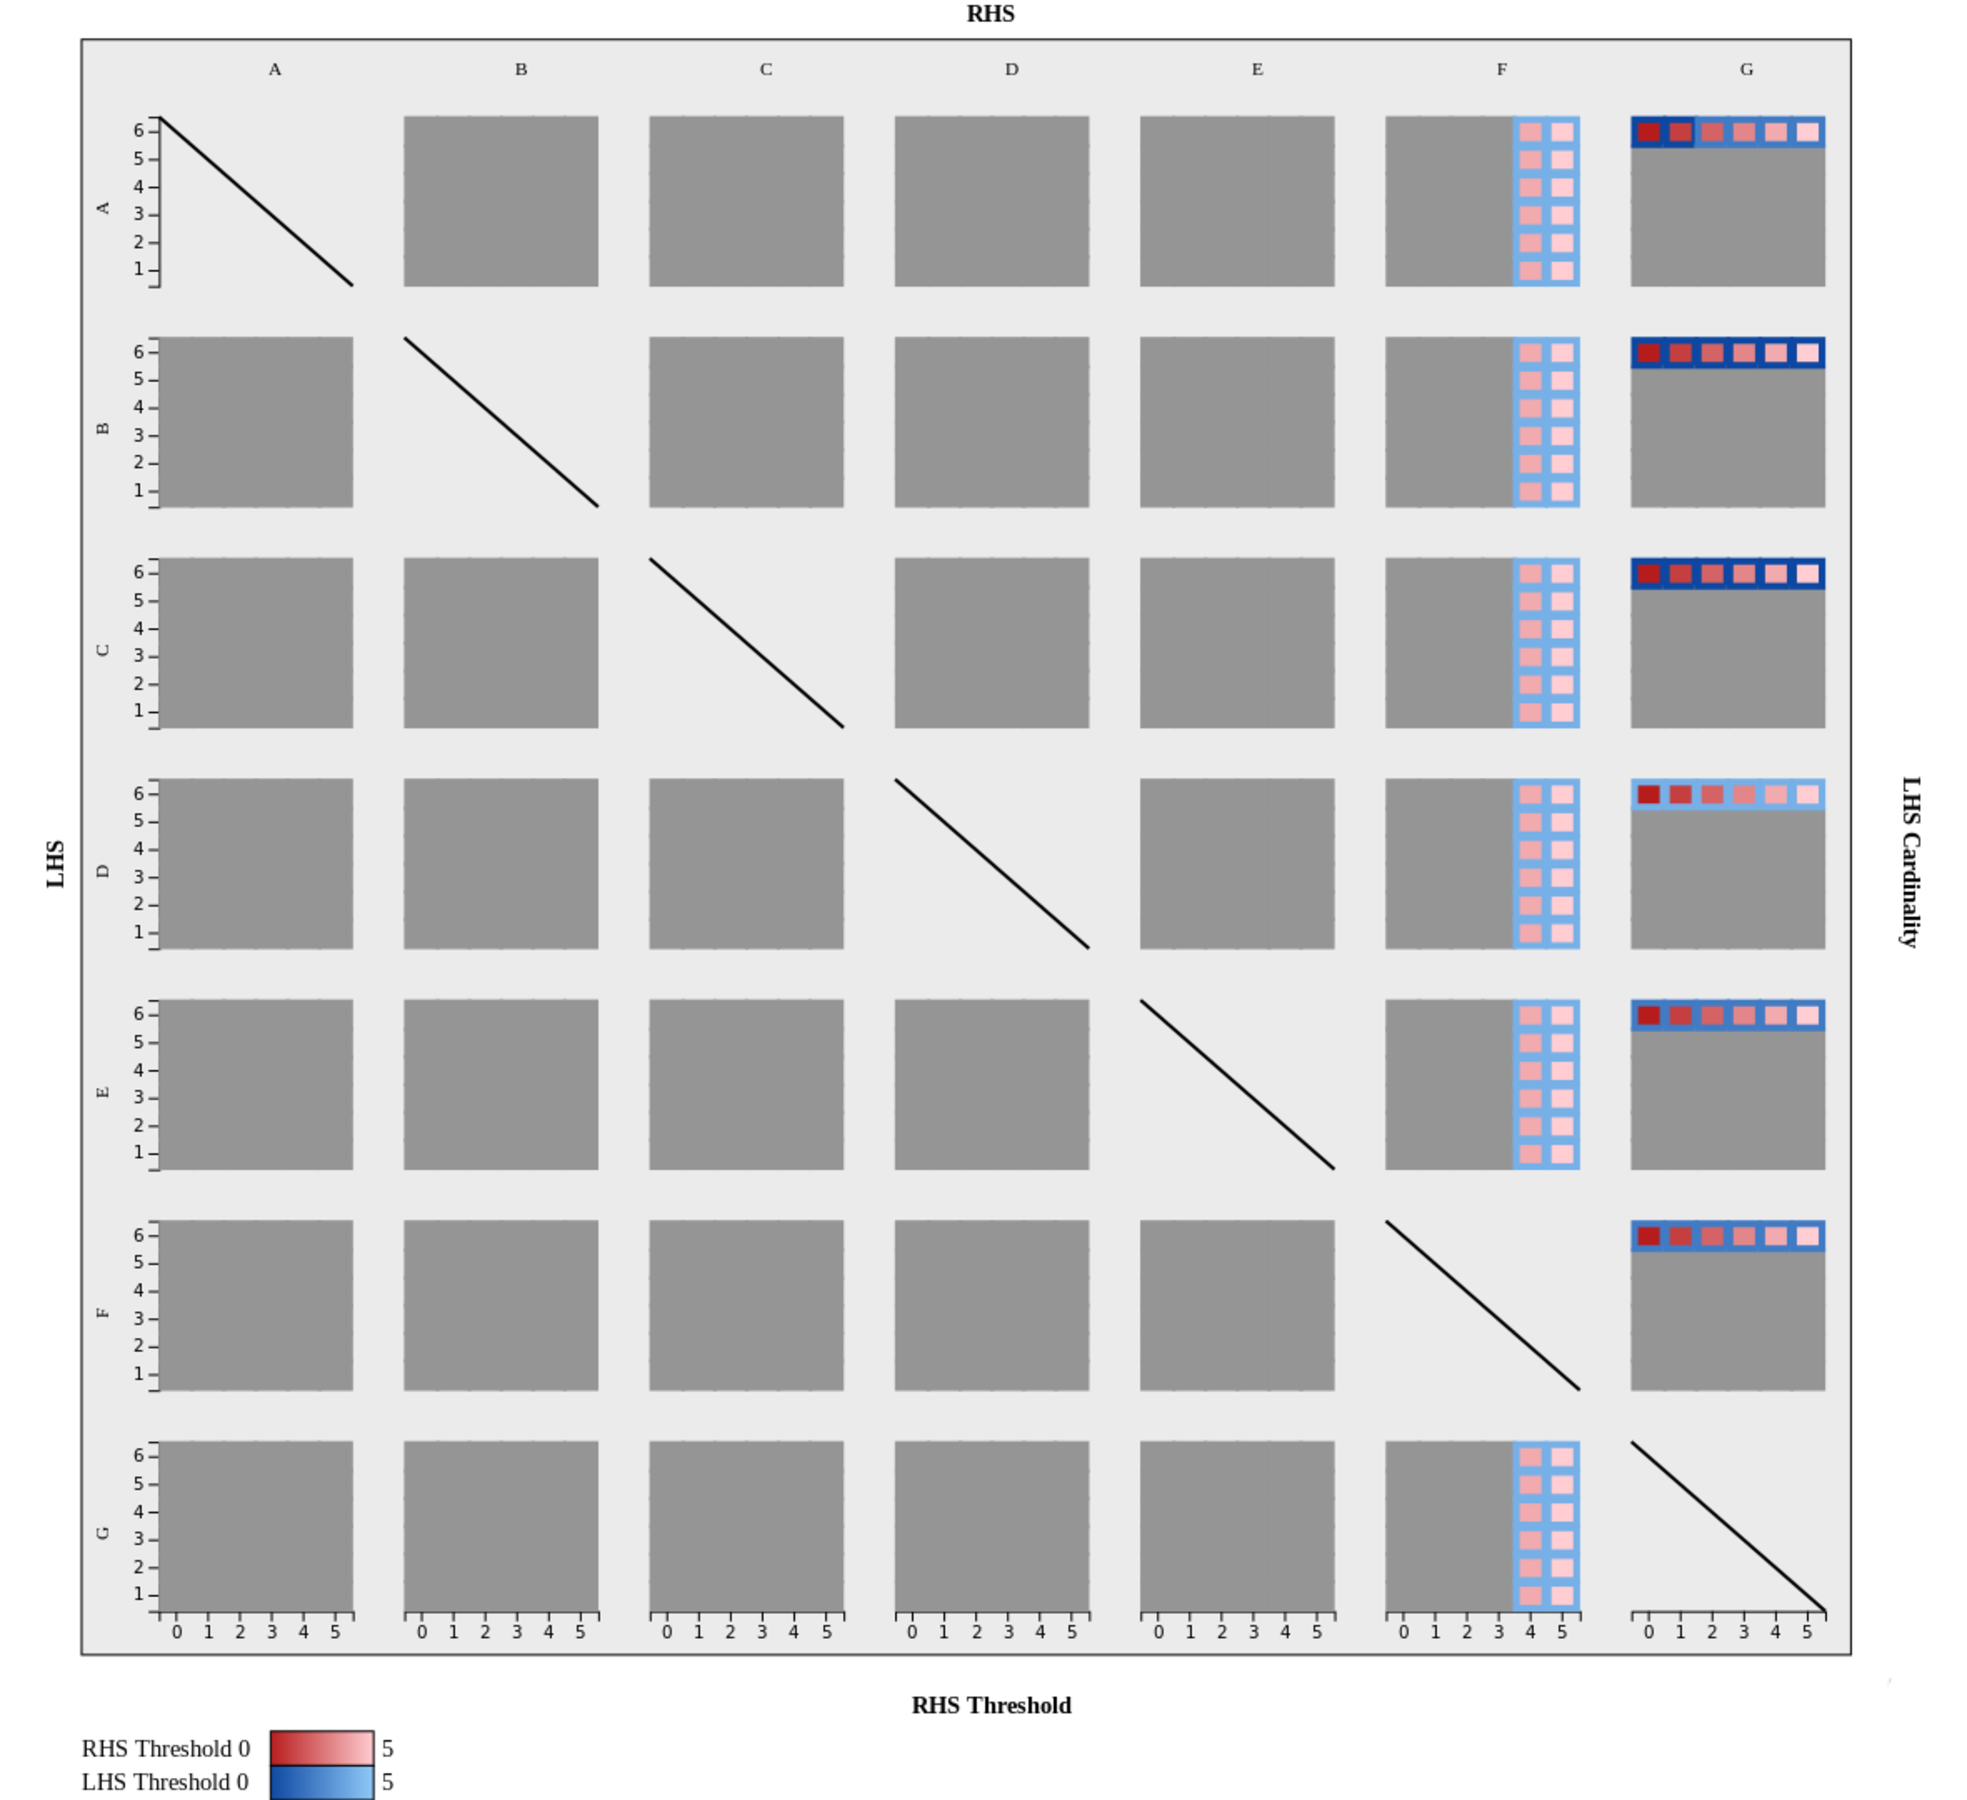
\includegraphics[width=\linewidth]{capitoli/figure/car_data}
    \caption{Rappresentazione ottenuta in output da Dependensee del dataset Car Data.}
    \label{fig:cardata_result}
\end{figure}
Il dataset \textit{Car\_Data} \`{e} stato analizzato con una soglia massima data in input pari a $5$. Le \acrlong{rfds} minimali presenti in questo dataset son poche e la maggior parte hanno una soglia alta. Se prendiamo in considerazione la colonna relativa all'attributo \texttt{F}, possiamo notare che le \acrlong{rfds} minimali esistenti siano tutte con una soglia sul lato sinistro pari a $5$ e soglia sul lato destro pari a $4$ e $5$. Se consideriamo, invece, la colonna relativa all'attributo \texttt{G}, possiamo notare che le \acrlong{rfds} minimali esistenti sono tutte con cardinalit\`{a} massima, con soglia massima o quasi sul lato sinistro e con soglia tra $0$ e $5$ sul lato destro.